\documentclass{article}
\usepackage{enumitem}
\usepackage[cachedir=minted_cache]{minted}
\usepackage{graphicx}
\graphicspath{ {./img/} }
\usepackage[margin=1in]{geometry} %used to set the margins
\setcounter{secnumdepth}{0} %used to get rid of section numbers
\title{Lab 8: \\ Tries and Dynamic Programming}
\author{Michael Morikawa}
\date{\today}


\begin{document}
\maketitle
\section{Lab Questions}
\begin{enumerate}[label=\textbf{Question \arabic*}]
      \item  Construct a Huffman coding tree for the following input string “more
            money”. Show the code for each character and include the total number of bits for the
            input string. \\
            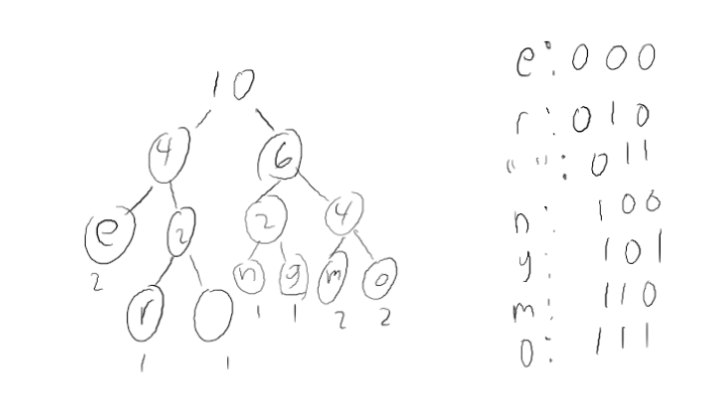
\includegraphics[scale=0.7]{Question_1.png} \\
            \textbf{
                  Input bits = 7*10 = 70
            }
      \item Lab question 2: Explain the main difference between standard tries and compressed
            tries. How much space is saved from standard tries to compressed tries?\\
            \textbf{
                  The difference between the two is that compressed tries make each internal node
                  have at least 2 children. Not much space is saved if you are simply storing the characters/substrings
                  and the nodes. You lessen the ammount of total nodes but the amount of data stored within the nodes is the same.
                  You can modify it to work with a collection of strings where you instead store a 3-tuple. The first
                  element is the index of the string, and the other 2 are the begin and end points of the string. This will
                  reduce the size from O(n), n = total length of strings, to O(s), s = number of strings.
            }


\end{enumerate}

\section{Source Code}

\subsection{main.cpp}
\inputminted{c++}{../src/main.cpp}

\section{Output}
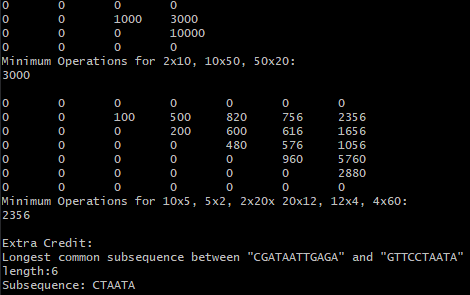
\includegraphics[]{output.png}

\end{document}